 
\documentclass[10pt]{article}

\usepackage[slovak]{babel}
\usepackage[utf8]{inputenc}
\usepackage[T1]{fontenc}
\usepackage{graphicx}

\usepackage{times}


\usepackage[margin=1in]{geometry} 
\usepackage{amsmath,amsthm,amssymb}
 
\newcommand{\N}{\mathbb{N}}
\newcommand{\Z}{\mathbb{Z}}
 
\newenvironment{theorem}[2][Theorem]{\begin{trivlist}
\item[\hskip \labelsep {\bfseries #1}\hskip \labelsep {\bfseries #2.}]}{\end{trivlist}}
\newenvironment{lemma}[2][Lemma]{\begin{trivlist}
\item[\hskip \labelsep {\bfseries #1}\hskip \labelsep {\bfseries #2.}]}{\end{trivlist}}
\newenvironment{exercise}[2][Exercise]{\begin{trivlist}
\item[\hskip \labelsep {\bfseries #1}\hskip \labelsep {\bfseries #2.}]}{\end{trivlist}}
\newenvironment{reflection}[2][Reflection]{\begin{trivlist}
\item[\hskip \labelsep {\bfseries #1}\hskip \labelsep {\bfseries #2.}]}{\end{trivlist}}
\newenvironment{proposition}[2][Proposition]{\begin{trivlist}
\item[\hskip \labelsep {\bfseries #1}\hskip \labelsep {\bfseries #2.}]}{\end{trivlist}}
\newenvironment{corollary}[2][Corollary]{\begin{trivlist}
\item[\hskip \labelsep {\bfseries #1}\hskip \labelsep {\bfseries #2.}]}{\end{trivlist}}
 
\begin{document}
 
% --------------------------------------------------------------
%                         Start here
% --------------------------------------------------------------
 
%\renewcommand{\qedsymbol}{\filledbox}
 
\title{TIN - Domáca úloha č. 3}%replace X with the appropriate number
\author{Roman Dobiáš - xdobia11@stud.fit.vutbr.cz}
 
\maketitle

\section*{Úloha č.1}
\subsection*{Identifikácia funkcie}
Zjavne sa jedná o \textit{Fibbonaciho postupnosť}. Páska č. 1 indikuje číslo N v zápise 1tiek, pre ktoré je funkcia Fib vypočítaná. Pásky 2 a 3 sľúžia na uchovanie predchádzajúcich dvoch
hodnôt postupnosti. 

Fibonačiho postupnosť je možné matematicky zadefinovať nasledujúco:
\begin{align}
    Fib(n) = 
    \begin{cases}
        0 & n = 0\\
        Fib(n-1) & n = 1\\
        Fib(n-1)\times Fib(n-2) & inak
    \end{cases}
\end{align}
\subsection*{Vyjadrenie funkcie pomocou primitívnej rekurzie}

Jedným z riešení je zaviesť pomocnú funkciu $K(x)$, ktorej vyčíslenie bude zodpovedať dvojici $(F(x), F(x+1)$ kde $F$ bude funkcia Fibbonaci.

Funkciu $K$ definujeme pomocou primitívnej rekurzie nasledujúco:

\begin{align*}
    K(0) &= \xi \times ( \sigma  \mathbin{o} \xi ) () \\
    K(x+1) &= \pi_3^3 \times (plus  \mathbin{o} ( \pi_2^3 \times \pi_3^3)  (x, K(x))
\end{align*}

Výpočet $K(0)$ je ekvivalentný návratovej dvojici $(0,1)$, ktorá zodpovedá hodnotám $(Fib(0), Fib(1))$. 
Následne pomocou primitívnej rekurzie má $K(x+1)$ sémantiku v tvare $K(x+1) = (Fib(x), Fib(x) + Fib(x-1))$, teda
$K(x+1) = (K(x).r, K(x).r + K(x).l)$, kde $l,r$ je ľavá, resp. práva hodnota dvojice.

Výsledná funkcia $F(x)$, ktorej hodnota je rovná Fibbonačiho postupnosti, má potom tvar:

\begin{align*}
    F(x) = (\pi_2^2 \mathbin{o} K) (x)
\end{align*}

\section*{Úloha č.2}
Diagonalizáciou ukážeme, že počet ohodnotení unárneho predikátu \textit{u} nad spočetným univerzom je nespočetný. Počet ohodnotení predikátu je totiž rovný $2^{\mathbb{N}}$, pretože pre každý prvok x z $\mathbb{N}$ prvkov univerza môžeme definovať $p(x)$ alebo $\neg p(x)$.
V dôkaze zároveň pracujeme s priradením, kde každej nulárnej funkcii $a_i$ priradíme hodnotu $i \in \mathbb{N}$.

\begin{proof}
    Predpokladajme, že počet realizácii je spočetný. Potom existuje bijektívne zobrazenie $f: \mathbb{N} \to P$, kde $P$ je množina realizácii.
    Jednotlivé realizácie môžeme vyjadriť ako nekonečný reťazec 0 a 1, ktorého jednotlivé symboly predstavujú ohodnotenie predikátu $p(i)$, kde $i \in \mathbb{N}$ je pozícia symbolu v reťazci, a teda ich môžeme usporiadať do nekonečnej postupnosti.
    Uvažujme nekonečnú maticu, kde $a_{ij}$ je 1 ak $a_j$ v realizácii $p_i$, alebo 0 ak $\neg a_j$ v realizácii $p_i$. Táto matica je znázornená v tabuľke č. 1.
\begin{table}[ht]
\begin{tabular}{l| lllll}
    & 1   & 2   & 3    & 4  & ... \\ \hline 
    $p_1$  & $a_{11}$ & $a_{12}$ & $a_{13}$  & $a_{14}$ &     \\
    $p_2$  & $a_{21}$ & $a_{22}$ & $a_{23}$  & $a_{24}$ &     \\
    $p_3$  & $a_{31}$ & $a_{32}$ & $a_{33}$  & $a_{34}$ &     \\
    $p_4$  & $a_{41}$ & $a_{42}$ & $a_{43}$  & $a_{44}$ &     \\
... &     &   &   &   &
\end{tabular}
    \caption{Nekonečná matica, znázorňujúca priradenie z $\mathbb{N}$ do $P$.}
\end{table}

Uvažujme realizáciu $p_c(x) = 1 - p_x(x)$. Táto realizácia sa od každej realizácie líši
    aspoň v jednom priradení a nenachádza sa teda medzi realizáciami $p_i, i \in \mathbb{N}$, ktoré sú uvedené v tabuľke, a zároveň, ktorých je spočetne. Zároveň táto realizácia je validnou realizáciou a patrí do množiny realizácii. To je spor, preto množina realizácii je nutne nespočetná. 
\end{proof}
\section*{Úloha č.3}
\begin{proof}
$\mathcal{O}(3^{2n}) \subseteq \mathcal{O}(2^{3n})$ \\
Z definície pre každú funkciu $f \in \mathcal{O}(3^{2n})$ platí, že $\exists c \in \mathbb{R}: \exists n_0 \in \mathbb{N}: \forall n \geq n_0: f(n) \leq c\times 3^{2n}$.  
Na to, aby $\mathcal{O}(3^{2n}) \subseteq \mathcal{O}(2^{3n})$ stačí ukázať, že každá funkcia $f \in \mathcal{O}(3^{2n})$ je ohraničená v $\mathcal{O}(2^{3n})$.

Predpokladajme, že platí práve spomenutý vzťah. Potom pre každú funkciu $f$ platí, že $\exists c,d \in \mathcal{R}^+: c \times 3^{2n} \leq d \times 2^{3n}$. 

Potom ale platia nasledujúce úpravy:

\begin{align*}
    c \times 3^{2n} \leq d \times 2^{3n}  \\
    1 \leq \frac{d \times 2^{3n}}{c \times 3^{2n}} \\
    1 \leq \frac{d}{c} \times \frac{2^{3n}}{3^{2n}} \\
    1 \leq \frac{d}{c} \times (\frac{2^{3}}{3^{2}})^n \\
    1 \leq \frac{d}{c} \times (\frac{8}{9})^n \\
\end{align*}
Platí, že $\lim_{n \to \infty} (\frac{8}{9})^n = 0$, teda platí, že $\lim_{n \to \infty} 1 \leq \frac{d}{c} \times (\frac{8}{9})^n  = 1 < 0$, čo je spor.
Preto neplatí $\mathcal{O}(3^{2n}) \subseteq \mathcal{O}(2^{3n})$.
\end{proof}

\begin{proof}
$\mathcal{O}(2^{3n}) \subseteq \mathcal{O}(3^{2n})$ \\
Z definície pre každú funkciu $f \in \mathcal{O}(2^{3n})$ platí, že $\exists c \in \mathbb{R}: \exists n_0 \in \mathbb{N}: \forall n \geq n_0: f(n) \leq c\times 2^{3n}$.  
Na to, aby $\mathcal{O}(2^{3n}) \subseteq \mathcal{O}(3^{2n})$ stačí ukázať, že každá funkcia $f \in \mathcal{O}(2^{3n})$ je ohraničená v $\mathcal{O}(3^{2n})$.

Predpokladajme, že platí práve spomenutý vzťah. Potom pre každú funkciu $f$ platí, že $\exists c,d \in \mathcal{R}^+: c \times 2^{3n} \leq d \times 3^{2n}$. 

Potom ale platia nasledujúce úpravy:

\begin{align*}
    c \times 2^{3n} \leq d \times 3^{2n}  \\
    1 \leq \frac{d \times 3^{2n}}{c \times 2^{3n}} \\
    1 \leq \frac{d}{c} \times \frac{3^{2n}}{2^{3n}} \\
    1 \leq \frac{d}{c} \times (\frac{3^{2}}{2^{3}})^n \\
    1 \leq \frac{d}{c} \times (\frac{9}{8})^n \\
\end{align*}
Ak zvolíme $d = c$, potom už pre $n = 0$ platí, že $1 \leq (\frac{9}{8})^n$.
Ukázali sme teda, že pre každú $f \in \mathcal{O}(2^{3n})$ sme schopný nájsť danú konštantu $d$ tak, aby $f$ bola ohraničená funkciou $\mathcal{O}(3^{2n})$.
Platí teda $\forall f \in \mathcal{O}(2^{3n}): f \in \mathcal{O}(3^{2n})$, teda platí $\mathcal{O}(2^{3n}) \subseteq \mathcal{O}(3^{2n})$. 
\end{proof}

\subsection*{Záver}
Platí $\mathcal{O}(2^{3n}) \subseteq \mathcal{O}(3^{2n})$, zároveň neplatí $\mathcal{O}(3^{2n}) \subseteq \mathcal{O}(2^{3n})$, preto neplatí ani $\mathcal{O}(3^{2n}) = \mathcal{O}(2^{3n})$


\section*{Úloha č.4}
Aby ste dokázali, že problém Tety Kvety je NP-úplný, ukážeme najskorej, že je možné skonštruovať NTS, ktorý overí, či inštancia problému Tety Kvety je platná. Zároveň ukážeme, že existuje redukcia z problému farbenia grafov, ktorý patrí do $NP$, na problém tety Kvety.


Problém tety kvety je možné charakterizovať ako jazyk Kveta = $\{$ w1 \# w2 \# k | w1 je postupnosť množstva nakúpených surovín, w2 je postupnosť jednotlivých pečív a množstva pre upečenie jedného kusu a K je počet priateľok a zároveň je možné upiecť aspoň k pečiv z dostupných surovín$\}$.
\subsection*{Prítomnosť Kveta v triede NP}
Pre problém tety Kvety existuje 3 páskový NTS M, ktorý v polynomiálnom čase uhádne riešenie a následne ho overí.
TS M bude pracovať nasledujúco:
\begin{itemize}
    \item TS M overí, či vstup w = w1\#w2\#k je validná inštancia jazyka \textit{Kveta}. Ak nie, TS M zamietne. Validnosť vstupu je možné vykonať konečným automatom, ktorého časová zložitosť je v $O(n)$. 
    \item TS M na pomocnú pásku nedeterministicky úhadne $k$ indexov, ktoré zodpovedajú jednotlivým pečivám, ktoré budú upečené. $O(n)$.
    \item TS M na ďalšiu pomocnú pásku skopíruje počet surovín $w1$  (v čase $O(n)$)
    \item TS M následne prechádza jednotlivé indexy pečív ($O(n)$) a pre každý z nich prechádza zoznam ingrediencii a postupne odčitáva ingrediencie od počtu dostupných surovín, ktoré má na pomocnej páske. Počet surovín pre dané pečivo je nejaké M, teda prejdenie zoznamu ingrediencii trvá $O(m)$. Dokopy trvá tento krok $O(m \times n )$.
 V prípade, že by pri odčítaní vzniklo záporné číslo, TS M odmietne.
    \item Nakoniec TS M prijme (ak nedošlo ku vzniku záporného čísla).
\end{itemize}

Ukázali sme, že existuje NTS, ktorý v polynomiálnom čase overí náležitosť $w$ do problému Tety Kvety. Problém Tety Kvety teda patrí do triedy $NP$.

\subsection*{Redukcia z Farbenia grafov na problém tety Kvety}

Rozhodovací problém farbenia grafov je jazyk ColorGraph = $\{$ (<V>,<E>\#k) | G = (<V>, <E>) je graf
ofarbitelný k farbami \}.
Redukcia z farbenia grafov na problem tedy Kvety je funkcia $\sigma$, pre ktorú existuje úplný DTS.
\subsection*{Algoritmus prevodu}
Každú inštanciu jazyka ColorGraph sme schopný previesť na problém Tety Kvety nasledujúco:
\begin{itemize}
    \item Pre každý uzol E vygenerujeme K+1 surovín, kde K je počet farieb a kde každá surovina má kapacitu 1 (teda, Teda
        Kveta má práve 1 inštanciu tejto suroviny). K surovín reprezentuje jednotlivé z K farieb a K+1 surovina
        je použitá pre detekovanie, či už je vrchol ofarbený.
        Jednotlivé z K+1 surovín označme ako $E_i, 0 \leq i \leq k$.
    \item Pre každé ofarbenie uzla E farbou F 
    \begin{itemize}
        \item vypočítame množinu vrcholov $I$ takých, že existuje hrana medzi vrcholom $E$ a vrcholom z
            $I$ a prizjednotíme vrchoľ $E$
        \item vytvoríme "pečivo" $E_F$, ktorého ingrediencie sú suroviny $a_i, a \in I, i = F$ a
            surovina $E_k$.
    \end{itemize}
    \item Pre takto zakódovaný problém riešime problém Tety Kvety pre počet priateľok $k$, kde $k = |V|$.
    \item Graf je ofarbiteľný práve vtedy, ak môžeme každý vrchol ofarbiť farbou tak, že
        priliehajúce vrcholy nemaju tú istú farbu.
    \item Zrejme platí, že ak upečiem pečivo $E_F$, potom toto pečivo bude pre daný vrchol jediné
        (vďaka surovine K+1, ktorá je dostupná pre daný vrchol len v jednej inštancii) a zároveň priliehajúce vrcholy nebudú mať rovnaké pečivo (farbu),
        pretože surovina ich farby už bola vyčerpaná pri pečení $E_F$.
    \item Teda platí, že ak je možné upiecť N rôznych pečív, kde N je počet vrcholov a zároveň
        platia tézy vyššie, potom graf je K-ofarbiteľný.
\end{itemize}

Platí, že graf $G$ je K-ofarbiteľný $\iff$ ku každému vrcholu V môžem priradiť farbu tak, že vrcholy na incidenčných hranách budú mať inú farbu $\iff$ môžem upiecť pečivo pre daný vrchol a počet upečených pečív je $|V|$.
\subsection*{Príklad}
Uvažujme graf A-B, B-C, C-D, D-A. Tento graf má chromatické číslo $k = 2$. 
Reprezentáciu úlohy môžeme vyjadriť tabulkou č.2. Hlavička predstavuje jednotlivé suroviny (pričomž z každej má teta Kveta len jednu inštanciu). Každému vrcholu grafu G zodpovedá 2+1 surovín.
V hlavičke stĺpcov sú uvedené jednotlivé pečivá, ktoré odpovedajú ofarbeniu daného vrcholu.

Zjavne jedným s riešením problému Tety Kvety je napiecť pečivá $A_0, B_1, C_0, D_1$, čo zodpovedá farbe 0 pre vrchol A, 1 pre B, 0 pre C a 1 pre D.

\begin{table}[ht]
\begin{tabular}{l|llllllllllll}
    & $A_0$ & $A_1$  &$A_2$  & $B_0$ &  $B_1$  &$B_2$ & $C_0$ &  $C_1$  &$C_2$  & $D_0$ & $D_1$  &$D_2$  \\ \hline
$A_0$  & X &  & X& X&  &  &  &  &  & X&  &  \\
$A_1$  &   & X& X&  & X&  &  &  &  &  & X&  \\
$B_0$  & X &  &  & X&  & X& X&  &  &  &  &  \\
$B_1$  &   & X&  &  & X& X&  & X&  &  &  &  \\
$C_0$  &   &  &  & X&  &  & X&  & X& X&  &  \\
$C_1$  &   &  &  &  & X&  &  & X& X&  & X&  \\
$D_0$  & X &  &  &  &  &  & X&  &  & X&  & X\\
$D_1$  &   & X&  &  &  &  &  & X&  &  & X& X 
\end{tabular}
    \caption{Príklad definície ingrediencii pre jednotlivé pečívá pre riešenie grafu G s k = 2}
\end{table}

\section*{Úloha č.5}
Nasledujúca PT Petriho sieť generuje jazyk $L = \{a^k(b^l)c^l | k \geq l \}$. \\
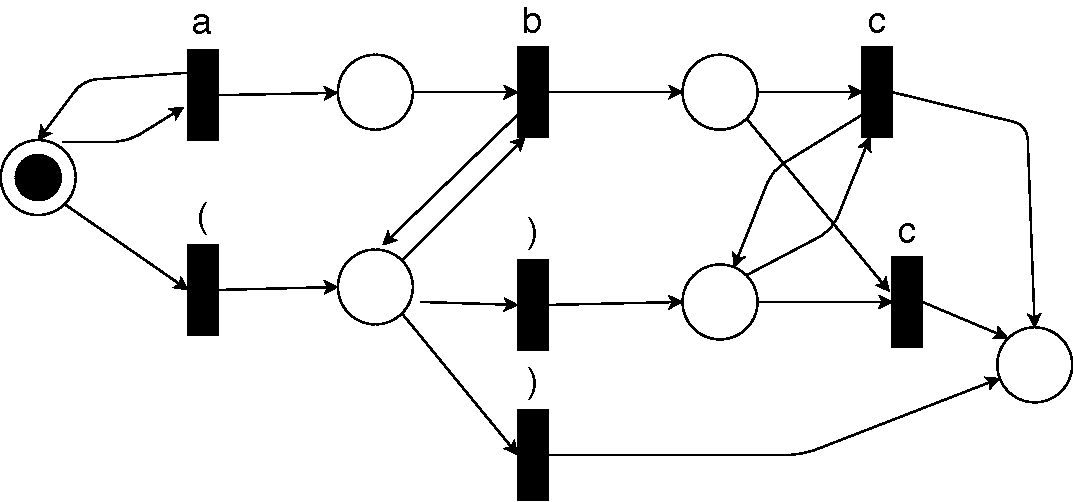
\includegraphics{petriNetFinalTake.pdf}

\end{document}
